\documentclass[11pt]{article}

\usepackage{amsmath}
\usepackage{textcomp}
\usepackage{float}
\usepackage[top=0.8in, bottom=0.8in, left=0.8in, right=0.8in]{geometry}
\usepackage{graphicx}
\usepackage{wrapfig}
\graphicspath{ {./} }
% Add other packages here %


% Put your group number and names in the author field %
\title{\bf Excercise 1.\\ Implementing a first Application in RePast: A Rabbits Grass Simulation.}
\author{Group \textnumero: 90  Kyle Gérard, Yann Bolliger}

\begin{document}
 \maketitle

 \section{Implementation}

\subsection{Assumptions}
\begin{itemize}

\item 
Our grass growth is bounded above linearly. We choose \texttt{grassGrowthRate} 
squares at each iteration tick and put grass on them. Regardless of whether 
there has already been grass or not. In that manner we add \textit{at most} \texttt{grassGrowthRate} 
new squares of grass at each tick.

\item 
The energy of the grass in a cell is always equal to \texttt{grassEnergy}.
This can be adjusted as a parameter.

 \item
 At birth, rabbits are placed at a random free cell. This can also be a cell 
 with grass in it.
 
 \item
  Rabbits loose one energy point at each tick. This is the case even if the rabbit is
  surrounded on all sides by other rabbits and can't move therefore.
  
  \item
   Rabbits move completely randomly. For each tick, each rabbit chooses among 
   the four possible directions and takes the first one that is not blocked by 
   another rabbit. This means that rabbits can also go back and forth.
   
   \item
   The first generation of rabbits that appear in the space at the start of the simulation
   have all a default birth energy of 30 points. 
\end{itemize}


 \subsection{Implementation Remarks}
 \begin{itemize}
   
   \item
   We added another user-facing  parameter: \texttt{grassEnergy}. All the 
 adjustable parameters are bounded  below by 0 but not above. Except for the 
 grid size that has to be at least 1.
 
 \item
 Another edge case is when a rabbit cannot move because it is surrounded by 
 other rabbits. In that case the rabbit will just stay where it is.
 
  \item
 Another edge case is when a rabbit cannot move because it is surrounded by 
 other rabbits. In that case the rabbit will just stay where it is.
 
 \end{itemize}
   


 \section{Results}

 \subsection{Experiment 1}
 \subsubsection{Setting}

 \begin{table}[H]
  \begin{tabular}{llll}
   &BirthThreshold  &10\\
   &GrassEnergy  &4 \\
   &GrassGrowthRate  &9\\
   &GridSize  &20*20\\
   &InitialNumberOfRabbits  &100
  \end{tabular}
 \end{table}
 
 \subsubsection{Observations}
 
 \begin{wrapfigure}{r}{0.5\textwidth}
  \vspace{-20pt}
  \begin{center}
    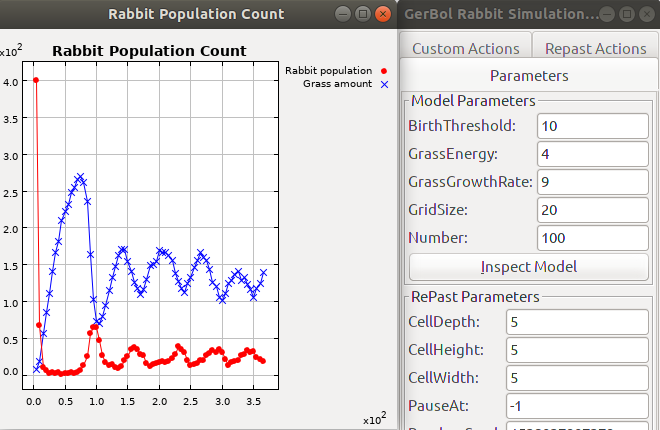
\includegraphics[width=0.48\textwidth]{exp1.png}
  \end{center}
  \vspace{-20pt}
\end{wrapfigure}
 
 These parameters are enough to sustain rabbit life with a population oscillating between 10 and 40 rabbits. This seems reasonable since 36 units of grass energy (GrassEnergy*GrassGrowthrate) are generated at every tick and each rabbit uses 1 unit of energy also at each step. Thus with this setting, the environment is not able to sustain more than 36 rabbits for long periods but is abundant in grass enough for some rabbits to survive.

 We remark that neither the grass amount nor the rabbit populations are stable but instead they oscillate periodically like a sinusoid. Their periods seem to be very similar, however they are inversely synchronized (when the rabbit population goes up, the grass amount goes down; when the rabbit population goes up, the grass amount goes down).


 \subsection{Experiment 2}
 \subsubsection{Setting}

 \begin{table}[H]
  \begin{tabular}{llll}
   &BirthThreshold  &40\\
   &GrassEnergy  &5 \\
   &GrassGrowthRate  &$x$ between 0 and 100\\
   &GridSize  &20*20\\
   &InitialNumberOfRabbits  &100
  \end{tabular}
 \end{table}

 \subsubsection{Observations}
 
  \begin{wrapfigure}{r}{0.5\textwidth}
  \vspace{-20pt}
  \begin{center}
    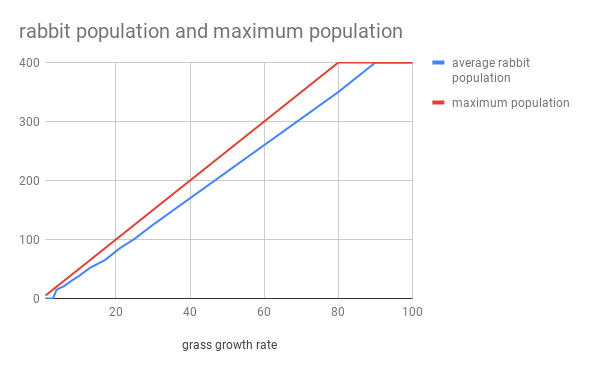
\includegraphics[width=0.48\textwidth]{grassgrowth.png}
  \end{center}
  \vspace{-20pt}
\end{wrapfigure}
 
 As seen in the graph above, the population of rabbits increases linearly in function of the GrassGrowthRate until the max number of rabbits is reached ( 400 which is the number of places on the 20*20 grid.

 The actual rabbit population follows closely the theoretical maximum sustainable population (GrassEnergy*GrassGrowthRate).


 \subsection{Experiment 3}
 \subsubsection{Setting}
 \begin{table}[H]
  \begin{tabular}{llll}
   &BirthThreshold  &40\\
   &GrassEnergy  & $$x$$ between 0 and 30 \\
   &GrassGrowthRate  &5\\
   &GridSize  &20*20\\
   &InitialNumberOfRabbits  &100
  \end{tabular}
 \end{table}

 \subsubsection{Observations}
  \begin{wrapfigure}{r}{0.5\textwidth}
  \vspace{-20pt}
  \begin{center}
    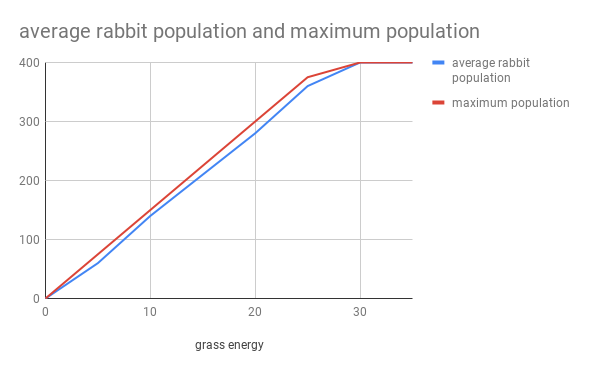
\includegraphics[width=0.48\textwidth]{grassenergy.png}
  \end{center}
  \vspace{-20pt}
\end{wrapfigure}

 As seen in the graph above and similarly to the previous experiment, the population of rabbits increases linearly in function of the grassEnergy until the max number of rabbits is reached ( 400 which is the number of places on the 20*20 grid.

 The actual rabbit population follows closely the theoretical maximum sustainable population (GrassEnergy*GrassGrowthRate).

 \subsection{Experiment 4}
 \subsubsection{Setting}
 \begin{table}[H]
  \begin{tabular}{llll}
   &BirthThreshold  &experiment a) 100 ; experiment b) 2\\
   &GrassEnergy  &5\\
   &GrassGrowthRate  &15\\
   &GridSize  &20*20\\
   &InitialNumberOfRabbits  &100
  \end{tabular}
 \end{table}

 \subsubsection{Observations}

 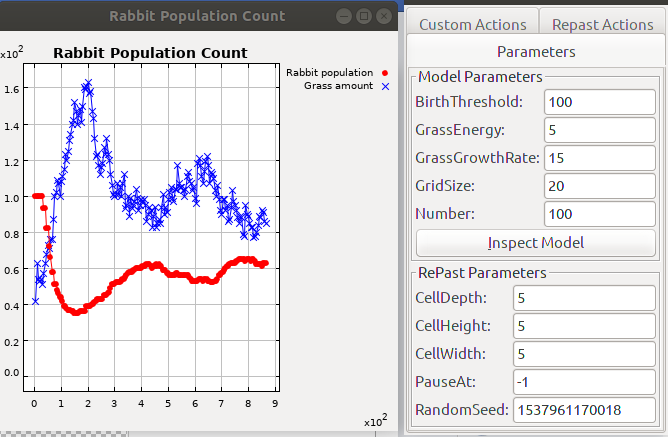
\includegraphics[width=0.48\textwidth]{slow_sinusoid.png}
 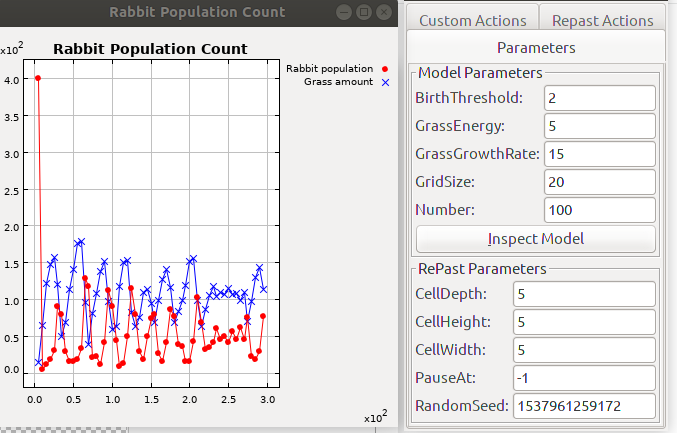
\includegraphics[width=0.48\textwidth]{fast_sinusoid.png}
 
 As seen in the above graphs, the periods of the sinusoid like rabbit population are much longer and its amplitude smaller with a high birth Threshold compared to a low one. Indeed, with a 100 BithThreshold we observe a period of around 200 steps and a amplitude of around 20 (population oscillates between 40 and 60 rabbits). With a 2 birthThreshold, the period is only  around 25 steps and the amplitude is above 90 (population oscillates between 10 and 100 rabbits).

\end{document}
